\documentclass[12pt,a4paper]{article}
\usepackage[a4paper,top=1.55cm,bottom=1.55cm,left=1.7cm,right=1.7cm]{geometry}
\usepackage{fontspec}
\setsansfont{Times New Roman}
\renewcommand{\familydefault}{\sfdefault}
\usepackage[french]{babel}
\usepackage{graphicx}
\usepackage[table]{xcolor}
\usepackage{booktabs}
\usepackage{tabularx}
\usepackage{array}
\usepackage{enumitem}
\usepackage{fancyhdr}
\usepackage{hyperref}
\usepackage{setspace}
\usepackage{titlesec}
\usepackage{tikz}
\usetikzlibrary{positioning,arrows.meta}
\usepackage{ragged2e}
\usepackage{caption}
\usepackage{float}

\definecolor{Navy}{HTML}{082F49}
\definecolor{Blue}{HTML}{075985}
\definecolor{Cyan}{HTML}{0E7490}
\definecolor{Orange}{HTML}{D97706}
\definecolor{Gold}{HTML}{FBBF24}
\definecolor{Ink}{HTML}{102A43}
\definecolor{Muted}{HTML}{52667A}
\definecolor{Pale}{HTML}{EFF8FB}
\definecolor{Line}{HTML}{D8E5EE}
\definecolor{SoftOrange}{HTML}{FFF7ED}

\hypersetup{colorlinks=true,linkcolor=Blue,urlcolor=Cyan,pdfauthor={Equipe SCO-RISKBurkina},pdftitle={SCO-RISK Burkina - Documentation de la solution}}
\setlength{\parindent}{0pt}
\setlength{\parskip}{5pt}
\setstretch{1.5}
\setlist[itemize]{leftmargin=5mm,itemsep=2.5pt,topsep=3pt}
\setlist[enumerate]{leftmargin=6mm,itemsep=3pt,topsep=3pt}
\renewcommand{\arraystretch}{1.22}
\titleformat{\section}{\Large\bfseries\color{Navy}}{}{0pt}{}
\titleformat{\subsection}{\large\bfseries\color{Blue}}{}{0pt}{}
\titlespacing*{\section}{0pt}{0pt}{7pt}
\titlespacing*{\subsection}{0pt}{8pt}{4pt}
\pagestyle{fancy}
\setlength{\headheight}{14pt}
\fancyhf{}
\fancyhead[LE,LO]{\small\color{Muted}SCO-RISK Burkina}
\fancyhead[RE,RO]{\small\color{Muted}Data Challenge Burkina 2026 - Défi 1}
\fancyfoot[C]{\small\color{Muted}\thepage}
\renewcommand{\headrulewidth}{0.3pt}
\renewcommand{\footrulewidth}{0pt}

% Ces deux liens seront renseignés après le déploiement final.
\newcommand{\GitHubURL}{https://github.com/kabreaziz60/SCO_RISKBURKINA-DATA-CHALENGE-BURKINA-SN-2026}
\newcommand{\DashboardURL}{}
\newcommand{\keybox}[2]{%
  \begin{minipage}[t]{0.48\linewidth}
  \colorbox{Pale}{\parbox{0.92\linewidth}{\vspace{2mm}\textbf{\color{Blue}#1}\\[-1mm]{\small #2}\vspace{2mm}}}
  \end{minipage}}
\newcommand{\note}[1]{\colorbox{SoftOrange}{\parbox{0.96\linewidth}{\textbf{\color{Orange}Point de vigilance.} #1}}}

\begin{document}

% Page 1 - couverture
\thispagestyle{empty}
\begin{tikzpicture}[remember picture,overlay]
  \fill[Navy] (current page.south west) rectangle (current page.north east);
  \fill[Cyan] (current page.south west) rectangle ([xshift=0.8cm]current page.north west);
  \fill[Orange] ([yshift=-0.35cm]current page.north west) rectangle ([yshift=-0.47cm]current page.north east);
\end{tikzpicture}
\color{white}
\vspace*{0.6cm}
\begin{center}
\colorbox{white}{\begin{minipage}{0.92\textwidth}
\centering\vspace{3mm}

\includegraphics[height=2.0cm]{../application/assets/armoiries_burkina_faso.png}\hfill

\includegraphics[height=1.55cm]{../application/assets/logo_africa_data_entry.jpg}\hfill

\includegraphics[height=1.55cm]{../application/assets/logo_semaine_numerique.png}
\vspace{3mm}
\end{minipage}}

\vspace{1.5cm}
{\large\bfseries DATA CHALLENGE BURKINA 2026}\par
\vspace{0.25cm}
{\color{Gold}\large 21e édition de la Semaine du numérique}\par
\vspace{1.35cm}
{\fontsize{34}{39}\selectfont\bfseries SCO-RISK Burkina}\par
\vspace{0.22cm}
{\large SCO : Système de Cartographie et d'Orientation}\par
{\large RISK : risque de décrochage scolaire}\par
\vspace{0.45cm}
{\Large Carte d'alerte et aide à la décision}\par
{\Large pour anticiper le risque de décrochage scolaire au primaire}\par
\vspace{1.2cm}
\colorbox{Orange}{\parbox{0.58\textwidth}{\centering\color{white}\Large\bfseries Défi 1 - Décrochage scolaire}}
\vfill
{\large\bfseries Équipe SCO-RISKBurkina}\par
\vspace{0.25cm}
{\normalsize Documentation de la solution - Novembre 2026}\par
\vspace{0.45cm}
{\small MTDPCE - Africa Data Entry}
\end{center}
\clearpage
\thispagestyle{fancy}
\color{Ink}

% Page 2
\section{Résumé exécutif et réponse au défi}
\textbf{Question du défi.} Où le risque de décrochage est-il le plus fort, par région, et comment l'anticiper ?

SCO-RISK transforme huit années de statistiques scolaires en un indice transparent, une carte provinciale et une projection prudente. En 2024-2025, les signaux les plus défavorables se concentrent notamment dans le Sahel, l'Est et le Nord. L'outil sert à organiser une revue humaine, prioriser les vérifications et suivre l'évolution territoriale ; il ne remplace pas la décision publique.

\vspace{4mm}
\keybox{8 années observées}{De 2017-2018 à 2024-2025, en respectant l'année scolaire.}\hfill
\keybox{360 observations}{45 provinces historiques suivies sur huit années.}

\vspace{3mm}
\keybox{Double référentiel}{13 régions et 45 provinces observées ; 17 régions et 47 provinces pour la projection.}\hfill
\keybox{Modèle évalué}{MAE de 9,55 contre 13,97 pour la référence naïve.}

\subsection{Utilisateurs et décisions soutenues}
Les directions centrales et régionales de l'éducation, les services statistiques et les responsables provinciaux peuvent utiliser la solution pour :
\begin{itemize}
  \item repérer les territoires à examiner rapidement ;
  \item comparer une province à son environnement régional et national ;
  \item distinguer un signal ponctuel d'une tendance persistante ;
  \item préparer une vérification de terrain avant toute allocation ou intervention.
\end{itemize}

\note{Le score mesure une priorité relative entre territoires. Il ne constitue ni une probabilité individuelle de décrochage ni une preuve de causalité.}
\clearpage

% Page 3
\section{Données, sources et confidentialité}
Les statistiques DGESS et les annuaires du primaire constituent le coeur de l'analyse. Les sources cartographiques servent à représenter correctement les unités administratives.

\begin{tabularx}{\textwidth}{>{\bfseries}p{3.5cm} X p{3.1cm}}
\rowcolor{Navy}\color{white}Source & \color{white}Usage & \color{white}Statut\\
DGESS 2016-2025 & Achèvement régional et séries principales & Source coeur\\
Annuaires du primaire & Abandon, redoublement et promotion par province et niveau & Source coeur\\
COD AB août 2025 & Limites des 17 régions et 47 provinces & Cartographie\\
ESU, PDI, EHCVM & Contexte potentiel pour une version future & Non intégré au score\\
\end{tabularx}

\subsection{Table d'analyse}
La table propre contient une ligne par province historique et année scolaire. Elle couvre 45 provinces et huit années, soit 360 observations. Chaque variable conserve sa source, son niveau géographique et son statut de qualité.

\subsection{Confidentialité appliquée}
\begin{itemize}
  \item traitements réalisés localement ;
  \item classeur original jamais modifié ;
  \item rapports détaillés conservés dans un dossier privé ;
  \item aucune donnée source transmise à un service d'intelligence artificielle ;
  \item dépôt public limité au code, à la documentation et aux éléments autorisés.
\end{itemize}

\subsection{Grain statistique}
Le grain retenu est \textbf{province - année scolaire}. Cette unité permet de suivre les tendances sans mélanger le primaire avec le préscolaire, le post-primaire ou le secondaire.
\clearpage
\thispagestyle{fancy}

% Page 4
\section{Parcours de traitement en cinq étapes}
La chaîne suit l'organisation demandée par le challenge et produit un livrable traçable à chaque étape.

\begin{center}
\begin{tikzpicture}[node distance=5mm]
\tikzset{processbox/.style={draw=Line,rounded corners=3pt,minimum width=15.6cm,minimum height=1.25cm,align=left,text width=14.8cm,fill=Pale}}
\node[processbox] (s1) {\textbf{01 Collecte}\quad Référencer les sources, inventorier les fichiers et sélectionner les tables du Défi 1.};
\node[processbox,below=of s1] (s2) {\textbf{02 Nettoyage}\quad Normaliser les provinces, retirer les totaux, contrôler les valeurs manquantes et documenter les anomalies.};
\node[processbox,below=of s2] (s3) {\textbf{03 Transformation}\quad Construire la table province-année, calculer les indicateurs et les correspondances géographiques.};
\node[processbox,below=of s3] (s4) {\textbf{04 Analyse}\quad Produire l'indice, tester sa sensibilité, évaluer le modèle et générer la projection.};
\node[processbox,below=of s4] (s5) {\textbf{05 Interprétation}\quad Cartographier les priorités, formuler les recommandations et construire la fiche décideur.};
\end{tikzpicture}
\end{center}

\begin{tabularx}{\textwidth}{>{\bfseries}p{3.2cm} X}
\toprule
Rôle & Production principale\\
\midrule
Data Engineer & Données propres, journal de nettoyage, scripts de construction\\
Data Architect & Référentiels, dictionnaire, organisation et circulation des données\\
Data Analyst & Indicateurs, comparaisons, carte et tableau de bord\\
Data Scientist & Modèle, mesure de fiabilité, projection et limites\\
\bottomrule
\end{tabularx}

Chaque notebook explique les choix en langage simple et conserve les contrôles qui permettent de reproduire le résultat.
\clearpage
\thispagestyle{fancy}

% Page 5
\section{Nettoyage et contrôles de qualité}
Le nettoyage conserve les valeurs sources, applique des règles explicites et signale les anomalies au lieu de les corriger silencieusement.

\begin{tabularx}{\textwidth}{X p{5.2cm}}
\rowcolor{Navy}\color{white}Contrôle & \color{white}Résultat\\
Unicité province et année scolaire & Aucun doublon sur 360 lignes\\
Complétude des composantes du score & Aucun score manquant\\
Plage des scores & Aucun score hors de 0 à 100\\
Cohérence promotion, redoublement et abandon & 1 800 triplets contrôlés\\
Anomalie de source & Une anomalie conservée, isolée et signalée\\
\end{tabularx}

\subsection{Règles humaines essentielles}
\begin{enumerate}
  \item L'année scolaire reste au format AAAA-AAAA et n'est jamais convertie en année civile.
  \item Les variantes d'écriture des provinces sont normalisées pour les jointures, tout en conservant le libellé source.
  \item Les lignes de total et les libellés parasites ne deviennent pas des provinces.
  \item L'achèvement régional reste étiqueté comme régional lorsqu'il apporte du contexte à une province.
  \item Toute correction est consignée dans le journal de nettoyage.
\end{enumerate}

\note{Les taux provinciaux sont des moyennes non pondérées des niveaux scolaires, faute de dénominateurs provinciaux compatibles dans les fichiers exploités.}
\clearpage
\thispagestyle{fancy}

% Page 6
\section{Piège géographique et solution retenue}
Les anciennes 13 régions et les nouvelles 17 régions ne se recoupent pas exactement. Le territoire national ne change pas, mais les regroupements administratifs changent. Réécrire tout l'historique dans le nouveau découpage créerait une fausse précision.

\begin{tabularx}{\textwidth}{p{3.2cm} p{4.8cm} X}
\rowcolor{Navy}\color{white}Période & \color{white}Affichage & \color{white}Principe\\
2017-2018 à 2024-2025 & 13 régions et 45 provinces & Respect des unités présentes dans les sources\\
Projection 2025-2026 & 17 régions et 47 provinces & Nouveau découpage avec correspondance documentée\\
\end{tabularx}

\subsection{Cas des nouvelles provinces}
Lorsque l'ancienne province du Soum ou de la Tapoa a été scindée, les nouvelles provinces reprennent le même signal historique faute de série distincte :
\begin{itemize}
  \item Djelgodji et Karo-Peli héritent de la série du Soum ;
  \item Dyamongou et Gobnangou héritent de la série de la Tapoa.
\end{itemize}

Une seule série source est comptée dans les synthèses afin d'éviter le double comptage. L'application affiche le statut \og hérité \fg{} ou \og non désagrégé \fg{}.

\note{La carte 2025-2026 est prospective. Elle ne prouve pas que chaque nouvelle province possède déjà un historique statistique autonome.}
\clearpage
\thispagestyle{fancy}

% Page 7
\section{Construction de l'indice de risque}
Chaque composante est transformée en rang percentile pour une même année scolaire. Cette normalisation rend les composantes comparables tout en conservant une lecture relative entre territoires.

\begin{center}
{\Large\bfseries\color{Blue}Score = 50\% abandon + 30\% redoublement + 20\% non-achèvement régional}
\end{center}

\begin{tabularx}{\textwidth}{>{\bfseries}p{4cm} p{2cm} X}
\rowcolor{Navy}\color{white}Composante & \color{white}Poids & \color{white}Interprétation\\
Abandon provincial & 50 \% & Signal le plus directement lié au décrochage\\
Redoublement provincial & 30 \% & Fragilité du parcours scolaire\\
Non-achèvement régional & 20 \% & Contexte partagé entre provinces d'une région\\
\end{tabularx}

\subsection{Seuils de lecture}
\begin{tabularx}{\textwidth}{p{3cm} p{3.5cm} X}
\toprule
Niveau & Score & Usage\\
\midrule
Faible & moins de 35 & Suivi courant\\
Modéré & 35 à moins de 55 & Surveillance\\
Élevé & 55 à moins de 75 & Revue prioritaire\\
Critique & 75 et plus & Vérification rapide\\
\bottomrule
\end{tabularx}

\subsection{Sensibilité des pondérations}
Deux pondérations alternatives ont été testées. La corrélation de rang minimale avec le classement principal est de 0,9403 et au moins huit provinces sur dix restent dans le groupe prioritaire. Le classement est donc relativement stable, sans être présenté comme une vérité absolue.
\clearpage
\thispagestyle{fancy}

% Page 8
\section{Résultats provinciaux observés en 2024-2025}
La lecture nationale fait apparaître un noyau de provinces à examiner en priorité. Les trois scores les plus élevés sont observés dans l'Oudalan, la Tapoa et la Kompienga.

\begin{figure}[H]
\centering
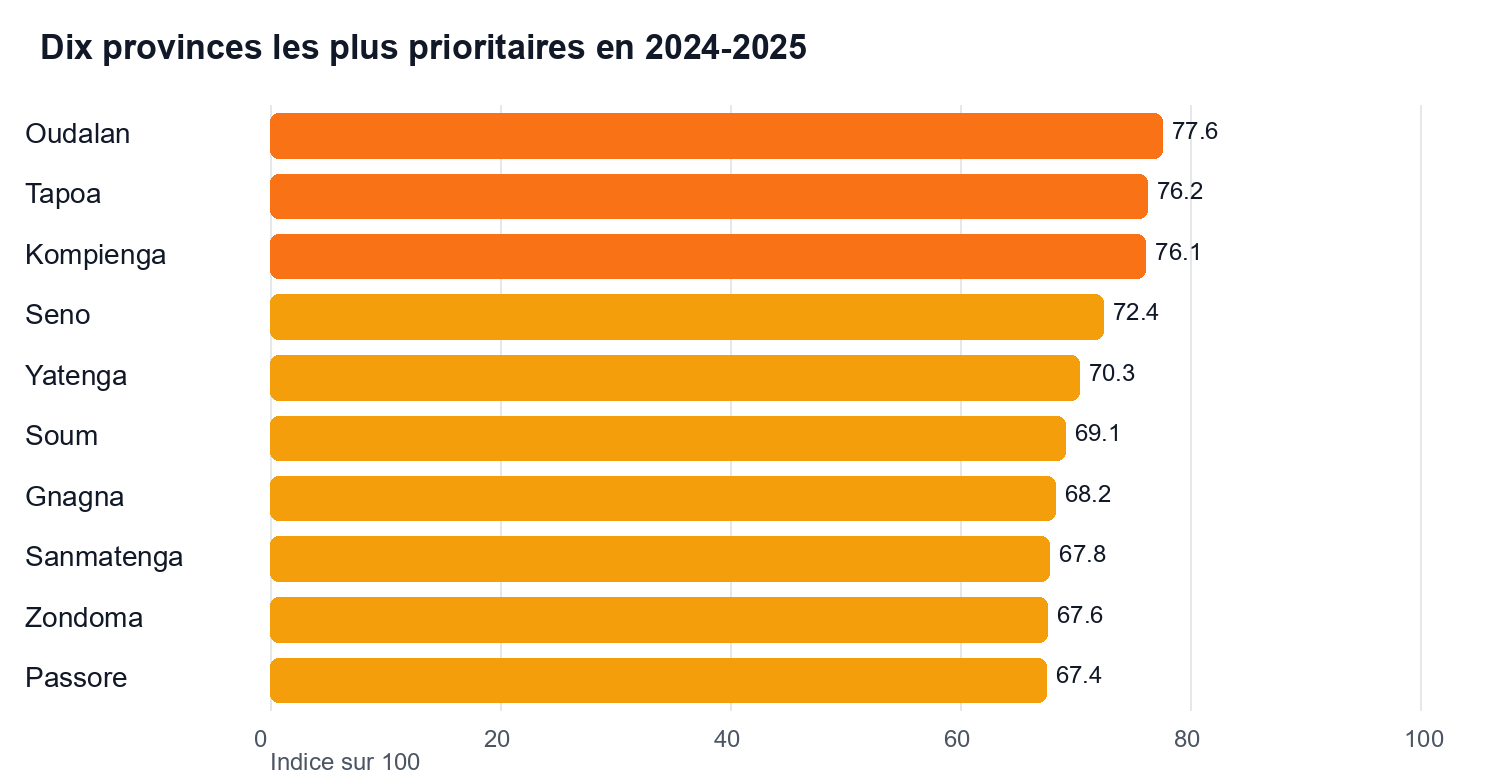
\includegraphics[width=0.94\textwidth]{assets/top10.png}
\caption*{Dix provinces affichant les scores les plus élevés.}
\end{figure}

\begin{tabularx}{\textwidth}{>{\bfseries}p{4.2cm} X}
Signal & Lecture pour la décision\\
\midrule
Score critique ou élevé & Vérifier rapidement les indicateurs et les événements locaux.\\
Hausse persistante & Comparer l'évolution des composantes et renforcer le suivi.\\
Facteur dominant & Orienter le diagnostic sans l'interpréter comme une cause démontrée.\\
\end{tabularx}
\clearpage
\thispagestyle{fancy}

% Page 9
\section{Lecture régionale et coordination territoriale}
La synthèse régionale permet de passer d'une priorité nationale à une coordination territoriale. Elle utilise la médiane des scores provinciaux afin de limiter l'influence des valeurs extrêmes.

\begin{figure}[H]
\centering
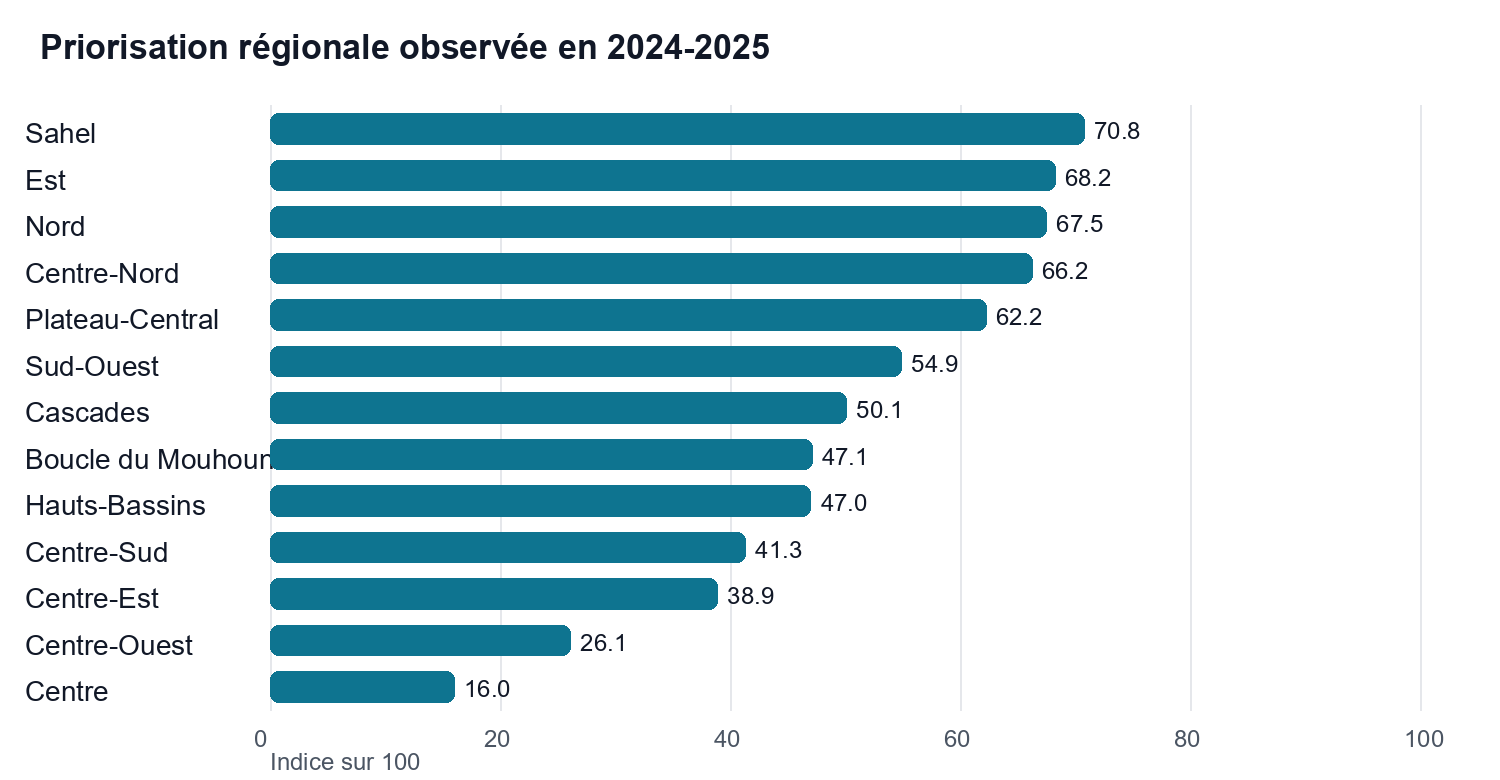
\includegraphics[width=0.94\textwidth]{assets/regions.png}
\caption*{Priorisation régionale observée en 2024-2025.}
\end{figure}

\begin{itemize}
  \item Le Sahel présente le score médian le plus élevé : 70,8 sur 100.
  \item L'Est atteint 68,2 et regroupe deux provinces critiques.
  \item Le Nord atteint 67,5 et concentre quatre priorités immédiates.
  \item Ces valeurs organisent l'ordre de revue ; elles ne démontrent pas les causes locales du décrochage.
\end{itemize}
\clearpage
\thispagestyle{fancy}

% Page 10
\section{Anticipation et mesure de fiabilité}
Le modèle Ridge prédit le score de l'année suivante à partir des informations disponibles avant la période cible. L'évaluation respecte le temps : apprentissage jusqu'en 2023-2024, puis test final sur 2024-2025.

\begin{tabularx}{\textwidth}{X p{3.6cm} p{3.6cm}}
\rowcolor{Navy}\color{white}Mesure sur 2024-2025 & \color{white}Référence naïve & \color{white}Modèle Ridge\\
Erreur absolue moyenne & 13,97 & \textbf{9,55}\\
Racine de l'erreur quadratique & 18,61 & \textbf{12,47}\\
Corrélation des rangs & 0,30 & \textbf{0,64}\\
Provinces communes dans le top 10 & 3 & \textbf{6}\\
\end{tabularx}

\subsection{Interprétation}
Le modèle réduit l'erreur absolue moyenne de 4,42 points par rapport à la référence naïve. Il est donc conservé pour la projection 2025-2026.

\subsection{Ce que la projection signifie}
Elle indique quels territoires méritent une vérification anticipée si les relations historiques se maintiennent. Elle ne prévoit ni un nombre d'élèves ni une probabilité individuelle.

\note{Toute alerte projetée doit être confrontée aux informations récentes sur les fermetures d'écoles, les déplacements, l'offre scolaire et les retours des services déconcentrés.}
\clearpage
\thispagestyle{fancy}

% Page 11
\section{Tableau de bord et carte interactive}
L'application Streamlit relie les filtres, la carte, le détail territorial et les recommandations dans une seule interface.

\begin{center}
\begin{tikzpicture}[node distance=8mm,>=Latex]
\tikzset{box/.style={draw=Line,rounded corners=4pt,fill=Pale,minimum width=4.4cm,minimum height=2.0cm,align=center,text width=4.0cm}}
\node[box] (f) {\textbf{Filtres}\\Année, région, province, seuil};
\node[box,right=of f] (m) {\textbf{Carte}\\Score, alerte et indicateurs au survol};
\node[box,right=of m] (d) {\textbf{Détail}\\Tendance, facteurs et actions};
\draw[-{Latex},thick,Blue] (f) -- (m);
\draw[-{Latex},thick,Blue] (m) -- (d);
\end{tikzpicture}
\end{center}

\subsection{Mode d'emploi}
\begin{enumerate}
  \item Choisir l'année scolaire. L'application utilise automatiquement le référentiel historique ou projeté.
  \item Choisir une région. La carte se recentre et met en évidence ses provinces.
  \item Choisir une province pour afficher son score, sa tendance et ses facteurs.
  \item Survoler une province sur la carte pour lire le score, l'alerte, l'abandon, le redoublement et l'achèvement régional.
  \item Ajuster le seuil pour modifier le nombre de provinces prioritaires.
  \item Cliquer sur \textbf{Réinitialiser les filtres} pour revenir à la vue nationale 2024-2025.
\end{enumerate}

Le zoom manuel est bloqué afin de conserver un cadrage stable. La projection 2025-2026 est signalée par un avertissement et n'est jamais présentée comme une observation.
\clearpage
\thispagestyle{fancy}

% Page 12
\section{Recommandations opérationnelles}
SCO-RISK organise une séquence de vérification et d'action. Il ne déclenche automatiquement ni sanction ni allocation.

\begin{tabularx}{\textwidth}{>{\bfseries}p{3.4cm} X}
\rowcolor{Navy}\color{white}Horizon & \color{white}Action proposée\\
Immédiat & Examiner les provinces critiques et élevées, confirmer les indicateurs et documenter les événements locaux.\\
Court terme & Croiser les alertes avec les fermetures d'écoles, les déplacements, l'offre scolaire et les retours des directions provinciales.\\
Suivi annuel & Comparer la position, la tendance et les facteurs dominants ; vérifier si l'action réduit durablement le signal.\\
Amélioration statistique & Ajouter des effectifs compatibles pour calculer des taux pondérés et distinguer les nouvelles provinces.\\
\end{tabularx}

\subsection{Questions à poser avant une action}
\begin{itemize}
  \item Le signal est-il confirmé par les données administratives les plus récentes ?
  \item Le facteur dominant reflète-t-il une réalité locale ou une limite de mesure ?
  \item La province projetée possède-t-elle une série propre ou hérite-t-elle d'une ancienne entité ?
  \item Quelle intervention est réaliste et comment son effet sera-t-il suivi ?
\end{itemize}

\note{La priorité est un point de départ pour le dialogue entre statisticiens, directions régionales, responsables provinciaux et acteurs de terrain.}
\clearpage
\thispagestyle{fancy}

% Page 13
\vspace*{1cm}
\section{Limites, éthique et précautions de décision}
\begin{tabularx}{\textwidth}{>{\bfseries}p{4.4cm} X}
\rowcolor{Navy}\color{white}Limite & \color{white}Conséquence\\
Moyennes non pondérées & Les taux ne reflètent pas exactement le poids des effectifs de chaque niveau.\\
Achèvement régional & Plusieurs provinces partagent la même composante contextuelle.\\
Deux scissions provinciales & Quatre nouvelles provinces reposent sur deux séries historiques sources.\\
Petit échantillon & La projection reste un outil de priorisation et non une prévision certaine.\\
Indice relatif & Un score élevé dépend aussi de la distribution nationale de l'année.\\
\end{tabularx}

\subsection{Garde-fous}
\begin{itemize}
  \item séparer visuellement les observations et les prévisions ;
  \item afficher la fiabilité et les limites avec le résultat ;
  \item ne pas descendre au niveau individuel ;
  \item conserver une validation humaine avant toute décision ;
  \item documenter les versions, les sources et les changements de référentiel.
\end{itemize}

\subsection{Améliorations futures}
L'ajout de dénominateurs provinciaux, de données récentes sur les fermetures d'écoles et les déplacements, ainsi qu'un suivi des interventions permettraient d'améliorer la pertinence du score et son évaluation.
\clearpage
\thispagestyle{fancy}

% Page 14
\section{Reproductibilité, conclusion et sources}
La solution se relance localement depuis les données autorisées jusqu'aux tests finaux.

\begin{center}
\colorbox{Pale}{\parbox{0.9\textwidth}{\ttfamily
Set-ExecutionPolicy -Scope Process -ExecutionPolicy Bypass\\
.\textbackslash scripts\textbackslash executer\_pipeline.ps1
}}
\end{center}

Cette commande reconstruit les données dérivées, contrôle la cohérence, recalcule l'indice, réévalue le modèle, produit les priorités et exécute 14 tests automatisés.

\subsection{Conclusion}
SCO-RISK répond au défi en localisant les signaux de décrochage, en montrant leur évolution et en proposant une anticipation évaluée. Sa valeur principale est la traçabilité : chaque alerte est reliée aux indicateurs, à l'année scolaire, au découpage administratif applicable et aux limites de la donnée.

\subsection{Sources principales}
\begin{itemize}
  \item DGESS, statistiques de l'éducation préscolaire et primaire 2016-2025 ;
  \item annuaires statistiques du primaire ;
  \item COD AB Burkina Faso, limites administratives, août 2025 ;
  \item Document du Data Challenge Burkina, édition Éducation 2026 ;
  \item Semaine du numérique 2026, thème officiel de la 21e édition.
\end{itemize}

\ifx\GitHubURL\empty\else\textbf{Code source :} \url{\GitHubURL}\\\fi
\ifx\DashboardURL\empty\else\textbf{Tableau de bord :} \url{\DashboardURL}\fi

\vfill
\begin{center}
{\large\bfseries\color{Blue}Une alerte pour mieux vérifier, comprendre et agir.}
\end{center}

\end{document}
